\documentclass[a4paper,11pt]{article}

%------------------------
% Taal & codering
%------------------------
\usepackage[english]{babel}        % Nederlandse hyphenatie en typografie
\usepackage[T1]{fontenc}         % Correcte font-encoding (accenten, afbreking)
\usepackage[utf8]{inputenc}      % Bronbestand in UTF-8 (met moderne LaTeX niet strikt nodig)
\usepackage{csquotes}            % Correcte aanhalingstekens (werkt goed met biblatex)

%------------------------
% Lettertype
%   XCharter + newtxmath geven een nette, consistente set
%------------------------
\usepackage{XCharter}            % Tekstfont
\usepackage[charter]{newtxmath} % Wiskunde bij Charter (variabele symbolen)
\usepackage{microtype}           % Mooiere microtypografie

%------------------------
% Wiskunde & symbolen
%------------------------
\usepackage{amsmath,mathtools}
\usepackage{siunitx}
\sisetup{
    per-mode = symbol,
    exponent-product = \cdot,
    output-decimal-marker = {.},
    exponent-product = \cdot
}
\DeclareSIUnit\phase{ph}  % Extra eenheid voorbeeld
\DeclareSIUnit{\ohmpsquare}{\text{\ensuremath{\Omega/\square}}}
\usepackage{nicematrix}

%------------------------
% Afbeeldingen, figuren, grafieken
%------------------------
\usepackage{graphicx}
\usepackage{wrapfig}
\usepackage{float}
\usepackage{subcaption}   % Vervangt subfig
\usepackage{pgfplots}
\usepackage{matlab-prettifier}
\usepgfplotslibrary{polar}
\pgfplotsset{compat=1.18}

%------------------------
% TikZ & elektrische schema's
%------------------------
\usepackage[european,american voltages]{circuitikz}
\usetikzlibrary{
  arrows.meta,
  positioning,
  shapes.geometric,
  patterns,
  backgrounds,
  scopes
}

%------------------------
% Tabellen en lijsten
%------------------------
\usepackage{booktabs,longtable,multirow,multicol,array}
\usepackage{tabularx}
\newcolumntype{Y}{>{\centering\arraybackslash}X}
\newcolumntype{?}{!{\vrule width 2pt}} % Dikke verticale lijn indien echt nodig
\newcommand{\thickhline}{\noalign{\hrule height 2pt}}

%------------------------
% Codefragmenten
%------------------------
\usepackage{listings}
\lstset{
  basicstyle=\ttfamily\small,
  frame=single,
  columns=fullflexible,
  showstringspaces=false,
  tabsize=2,
  breaklines=true,
  language=C
}

\definecolor{codegreen}{rgb}{0,0.5,0}
\definecolor{codegray}{rgb}{0.5,0.5,0.5}
\definecolor{codepurple}{rgb}{0.58,0,0.82}
\definecolor{backcolour}{rgb}{0.97,0.97,0.97}

\lstdefinestyle{mypython}{
    language=Python,
    backgroundcolor=\color{backcolour},
    basicstyle=\ttfamily\scriptsize,
    keywordstyle=\color{blue},
    commentstyle=\color{codegreen},
    stringstyle=\color{codepurple},
    numberstyle=\tiny\color{codegray},
    numbers=left,
    numbersep=6pt,
    breaklines=true,
    breakatwhitespace=false,
    showstringspaces=false,
    showspaces=false,
    showtabs=false,
    tabsize=4,
    frame=single,
    captionpos=b,
    keepspaces=true
}

%------------------------
% Verwijzingen & hyperlinks (volgorde: eerst hyperref, dan cleveref)
%------------------------
\usepackage[hidelinks]{hyperref}
\usepackage[noabbrev,nameinlink]{cleveref}

\usepackage{attachfile2}

%------------------------
% Opmaak & randvoorwaarden
%------------------------
\usepackage{parskip}      % Geen inspringing, wel witregel tussen alinea's
\usepackage{enumitem}     % Fijnere controle lijsten
\usepackage{xcolor}
\usepackage{fancyhdr}
\usepackage{geometry}
\geometry{
  a4paper,
  left=30mm,right=30mm,top=33mm,bottom=20mm
}
\pagestyle{fancy}
\fancyhf{}
\lhead{\leftmark}
\rhead{\thepage}

%------------------------
% Bibliografie (IEEE-stijl, biber-backend)
%------------------------
\usepackage[
  backend=biber,
  bibstyle=ieee,
  citestyle=numeric-comp,
  doi=false,isbn=false,url=true
]{biblatex}
\addbibresource{references.bib}

%------------------------
% Caption-breedte en centrering
%------------------------
\usepackage[justification=centering]{caption}
\captionsetup{width=0.95\linewidth}

%------------------------
% Handige eigen omgevingen/lijsten
%------------------------
\newlist{requirements}{enumerate}{10}
\setlist[requirements]{label*=REQ-\arabic*,leftmargin=*,itemsep=0.25em}

\newlist{Nreq}{enumerate}{10}
\setlist[Nreq]{label*=NREQ-\arabic*,leftmargin=*,itemsep=0.25em}

\newlist{research}{enumerate}{10}
\setlist[research]{label*=RQ-\arabic*,leftmargin=*,itemsep=0.25em}

%------------------------
% Bestandslocaties voor afbeeldingen
%------------------------
\graphicspath{{./figures/}}

% Optioneel: euroteken (meestal overbodig met moderne fonts)
% \usepackage{eurosym}

% Optioneel: PDF inladen
% \usepackage{pdfpages}

% Optioneel: externe referenties
% \usepackage{xr}

\mathchardef\Re="023C
\mathchardef\Im="023D

\DeclareSIUnit{\dBi}{dBi}
\DeclareMathOperator{\sinc}{sinc}

\usepackage{titlesec}
\usepackage{tocloft}
\setlength{\cftsubsecnumwidth}{2.25cm}

\renewcommand{\thesubsection}{Question \arabic{subsection}}

\titleformat{\subsection}
{\normalfont\large\bfseries}
{\thesubsection}
{1cm}
{}

\renewcommand{\cftdot}{}

\title{Modelling of Dynamical Systems \\ \small{3D printer}}
\author{Erwin den Boer (5513324)\\Group 61}
\date{\today}

\begin{document}
\maketitle

\newpage

\tableofcontents

\par\noindent\rule{\textwidth}{0.4pt}

\section{Introduction}

The mini-project involves the modelling of a 3D-printer in three different domains.
The domains are Physical, Discrete, and Hybrid.
In \Cref{fig:3D-printer} the schematic overview with the associate variable names and orientations are shown. The orientation and names of the corresponding physical quantity are respected in the derivation of the models. The mandatory variable names are given in \Cref{tab:variables}. The formulas contain auxiliary variables which may not be given in this table. 

\begin{figure}[H]
    \centering
    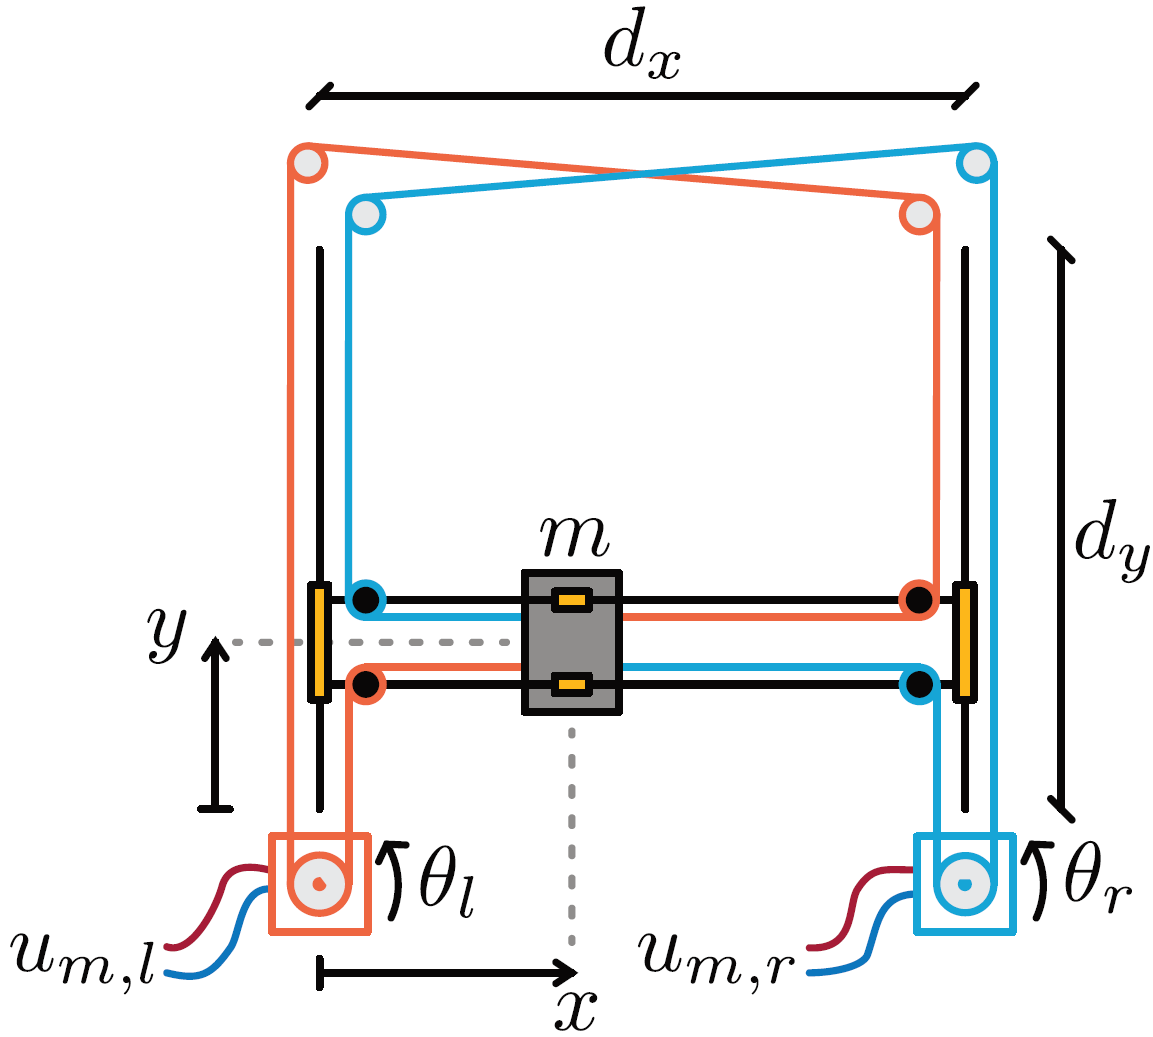
\includegraphics[width=0.68\linewidth]{3D-printer.png}
    \caption{The schematic view of the 3D-printer.}
    \label{fig:3D-printer}
\end{figure}

\clearpage
\begin{table}[p]
    \centering
    \caption{Variables and parameters of the 3D-printer.}
    \label{tab:variables}

    \begingroup
    \small
    \renewcommand{\arraystretch}{1.18}
    \sisetup{
        per-mode = symbol,
        output-decimal-marker = {.}
    }

    \begin{tabular}{
        @{}
        l
        @{\hspace{1.5em}}
        c
        @{\hspace{1.5em}}
        S[table-format=3.3]
        @{\hspace{0.8em}}
        l
        @{}
    }
        \toprule
        \textbf{Name}
            & \textbf{Symbol}
            & {\textbf{Value}}
            & \textbf{Unit} \\
        \midrule

        \multicolumn{4}{@{}l}{\textit{Motors and print head}} \\
        \addlinespace[3pt]
        Motor angle left
            & $\theta_l$ & & \unit{\radian} \\
        Motor voltage left
            & $u_{m,l}$ & & \unit{\volt} \\
        Motor current left
            & $i_{m,l}$ & & \unit{\ampere} \\
        Motor radius
            & $r_m$ & 11 & \unit{\milli\metre} \\
        Motor inductance
            & $L_m$ & 10 & \unit{\milli\henry} \\
        Motor resistance
            & $R_m$ & 90 & \unit{\ohm} \\
        Motor inertia
            & $J_m$ & \multicolumn{1}{c}{\num{8e-6}} & \textemdash \\
        Motor constant
            & $K_m$ & 0.07
            & \unit{\newton\metre\per\ampere} \\
        Tool head position
            & $x,y$ & & \unit{\metre} \\
        Tool head mass
            & $m$ & 60 & \unit{\gram} \\

        \addlinespace[6pt]
        \multicolumn{4}{@{}l}{\textit{Nozzle and thermal parameters}} \\
        \addlinespace[3pt]
        Nozzle voltage
            & $u_n$ & & \unit{\volt} \\
        Nozzle current
            & $i_n$ & & \unit{\ampere} \\
        Nozzle capacitance
            & $C_n$ & & \unit{\farad} \\
        Nozzle thermal capacity
            & $C_{t,n}$ & & \unit{\joule\per\kelvin} \\
        Nozzle thermal resistance
            & $R_{t,n}$ & 9 & \unit{\kelvin\per\watt} \\
        Nozzle resistance
            & $R_n$ & 8 & \unit{\ohm} \\
        Nozzle temperature
            & $T_n$ & 240 & \unit{\degreeCelsius} \\
        Environmental temperature
            & $T_e$ & 300 & \unit{\kelvin} \\

        \addlinespace[6pt]
        \multicolumn{4}{@{}l}{\textit{Bearing friction}} \\
        \addlinespace[3pt]
        Rolling bearing friction
            & $\mu_r$ & 0.003
            & \unit{\newton\second\per\metre} \\
        Linear bearing friction, $x$-direction
            & $\mu_{l,x}$ & 0.002
            & \unit{\newton\second\per\metre} \\
        Linear bearing friction, $y$-direction
            & $\mu_{l,y}$ & 0.001
            & \unit{\newton\second\per\metre} \\

        \addlinespace[6pt]
        \multicolumn{4}{@{}l}{\textit{Print bed and geometry}} \\
        \addlinespace[3pt]
        Print bed temperature
            & $T_b$ & 105 & \unit{\degreeCelsius} \\
        Print area dimension, $x$-direction
            & $d_x$ & 29 & \unit{\centi\metre} \\
        Print area dimension, $y$-direction
            & $d_y$ & 29 & \unit{\centi\metre} \\

        \bottomrule
    \end{tabular}

    \par\medskip
    \begin{minipage}{0.95\linewidth}
        \footnotesize
        Right motor variables are analogous to those of the left motor.
        Empty value cells indicate variables or unspecified parameters.
        The unit of motor inertia is not specified in the assignment.
    \end{minipage}
    \endgroup
\end{table}
\clearpage

\section{Physical Modelling}

\subsection{Kinematics}

The displacement of the belt by the driving motors having a radius of $r_m$ can be expressed by the following equation
\begin{equation}
    \Delta s = r_m \Delta \theta.
\end{equation}

The leads to the equations for the left and right motor being described by 
\begin{align}
    r_m \Delta \theta_l &= \Delta x + \Delta y\\
    r_m \Delta \theta_r &= \Delta x - \Delta y.
\end{align}

In order to find $\Delta x$, one could add both equations 
\begin{align}
    \left(\Delta x + \Delta y\right) + \left(\Delta x - \Delta y\right) &= r_m \Delta \theta_l + r_m \Delta \theta_r,\\
    2 \Delta x &= r_m \left(\Delta \theta_l +\Delta \theta_r \right),\\
    \Delta x &= \frac{r_m}{2} \left(\Delta \theta_l +\Delta \theta_r \right).
\end{align}

Similarly, the equation for $\Delta y$ can be found by substraction
\begin{align}
    \left(\Delta x + \Delta y\right) - \left(\Delta x - \Delta y\right) &= r_m \Delta \theta_l - r_m \Delta \theta_r,\\
    2 \Delta y &= r_m \left(\Delta \theta_l - \Delta \theta_r \right),\\
    \Delta y &= \frac{r_m}{2} \left(\Delta \theta_l -\Delta \theta_r \right).
\end{align}

When the reference is taken to be zero (i.e., $x_0,y_0,\theta_{l,0},\theta_{r,0}=0$), the prefix $\Delta$ can be discarded. The earlier derived equations simplifies to
\begin{align}
    x &= \frac{r_m}{2} \left(\theta_l + \theta_r \right),\\
    y &= \frac{r_m}{2} \left(\theta_l - \theta_r \right).
\end{align}

The velocities can be found by differentiation
\begin{align}
    \dot{x} &= \frac{r_m}{2} \left(\dot{\theta_l} + \dot{\theta_r}\right),\\
    \dot{y} &= \frac{r_m}{2} \left(\dot{\theta_l} - \dot{\theta_r}\right).
\end{align}

The rotational speed is given by the derivative of the angle (i.e., $\dot{\theta}=\omega$). Therefore, the velocities can alternatively be denoted by
\begin{align}
    \dot{x} &= \frac{r_m}{2} \left(\omega_l + \omega_r\right),\\
    \dot{y} &= \frac{r_m}{2} \left(\omega_l - \omega_r\right).
\end{align}

\subsection{Dynamics}

The model of the DC motor coupled to a disk with an inertia is shown in \Cref{fig:DC-motor}.
\begin{figure}[H]
    \centering
    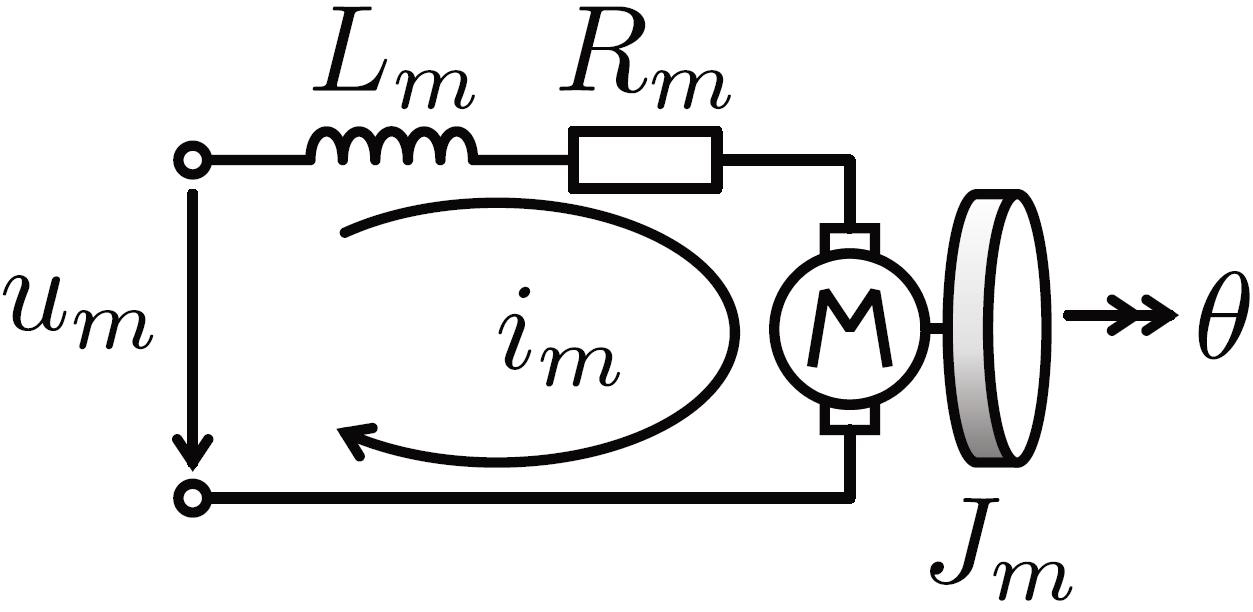
\includegraphics[width=0.7\linewidth]{DC-motor.png}
    \caption{The proposed DC motor modelled as an LR circuit.}
    \label{fig:DC-motor}
\end{figure}

Applying Kirchhoff's voltage law on the schematic of \Cref{fig:DC-motor} leads to\footnote{The derivative is normally denoted by a dot $\left(\text{e.g., }\dot{\theta}\right)$ in this assignment except when the differential quantity is current $\left(\text{i.e., }i\right)$. In that case, the explicit notation is used $\left(\text{i.e., }\frac{di}{dt}\right)$ in order to avoid confusion using a double dot $\left(\text{i.e., }\dot{i}\right)$.}
\begin{align}
    u_m &= u_{L_m} + u_{R_m} + u_{\text{EMF}}\\
    u_m &= L_m \frac{di}{dt} + R_m i + K_m \dot{\theta}\\
    \frac{di}{dt} &= - \frac{R_m}{L_m}i - \frac{K_m}{L_m}\omega + \frac{1}{L_m}u_m
\end{align}

The rotation of the disc and its inertia is related to the current flowing through the motor.
\begin{align}
    \tau &= K_m i \\
    \tau &= J \dot{\omega}\\
    \dot{\omega} &= \frac{K_m}{J}i.
\end{align}

The states are chosen as
\begin{align}
    \mathbf{x} &= \left[\theta_l \, \theta_r \, \omega_l \, \omega_r \, i_{m,l} \, i_{m,r}\right]^{\mathsf{T}}.
\end{align}

The input vector is defined by
\begin{align}
    \mathbf{u} &= \left[u_{m,l} \, u_{m,r}\right]^{\mathsf{T}}.
\end{align}

The positions of the 3D-printer are selected as the output vector of the system 
\begin{align}
    \mathbf{y} = \left[x \, y\right]^{\mathsf{T}}.
\end{align}

Therefore, leading to the elaborate state-space description 
\begin{equation}
\begingroup
\renewcommand{\arraystretch}{1.25}
\begin{aligned}
    \dot{\mathbf{x}}
    &=
    \underbrace{
        \begin{bNiceMatrix}[columns-width=9mm]
            0 & 0 & 1 & 0 & 0 & 0 \\
            0 & 0 & 0 & 1 & 0 & 0 \\
            0 & 0 & 0 & 0
                & \frac{K_{m,l}}{J_l} & 0 \\
            0 & 0 & 0 & 0
                & 0 & \frac{K_{m,r}}{J_r} \\
            0 & 0 & -\frac{K_{m,l}}{L_{m,l}} & 0
                & -\frac{R_{m,l}}{L_{m,l}} & 0 \\
            0 & 0 & 0 & -\frac{K_{m,r}}{L_{m,r}}
                & 0 & -\frac{R_{m,r}}{L_{m,r}}
        \end{bNiceMatrix}
    }_{\mathbf{A}}
    \,\mathbf{x}
    +
    \underbrace{
        \begin{bNiceMatrix}[columns-width=9mm]
            0 & 0 \\
            0 & 0 \\
            0 & 0 \\
            0 & 0 \\
            \frac{1}{L_{m,l}} & 0 \\
            0 & \frac{1}{L_{m,r}}
        \end{bNiceMatrix}
    }_{\mathbf{B}}
    \,\mathbf{u}
    \\[2em]
    \mathbf{y}
    &=
    \underbrace{
        \begin{bNiceMatrix}[columns-width=9mm]
            \frac{r_m}{2} & \frac{r_m}{2}
                & 0 & 0 & 0 & 0 \\
            \frac{r_m}{2} & -\frac{r_m}{2}
                & 0 & 0 & 0 & 0
        \end{bNiceMatrix}
    }_{\mathbf{C}}
    \,\mathbf{x}.
\end{aligned}
\endgroup
\end{equation}

\subsection{Decouple the x and y dynamics}

\subsection{Drawing shapes}

\subsection{Model the Nozzle}

\subsection{Printing a circle of filament (PDE)}

\section{Finite State Machine}

\subsection{Finite State Machines — Filament replacement}

\subsection{Automata — Parked detection}

\section{Hybrid system}

\subsection{Filament replacement}

\subsection{Draw a square}

\end{document}